\documentclass[a4paper,10pt]{article}
\usepackage{geometry,gretlhds}
\usepackage{url,fancyvrb}
\usepackage{pifont}
\usepackage[utf8]{inputenc}
\usepackage[pdftex]{graphicx}
\usepackage{color}
\usepackage{dcolumn,amsmath,mathrsfs}
%\usepackage{bm,bbm}
\usepackage{bm}
\usepackage{natbib}
%\bibliographystyle{apalike2}
\bibliographystyle{gretl}

%\graphicspath{{graphs/}}

\newenvironment{funcdoc}[1]
{\noindent\hrulefill\newline\texttt{#1}\par\noindent\hrulefill\par\medskip\par}
{\bigskip}

% ---------- Ripped from gretl.sty ----------------------------------------

\newcommand{\scriptname}{Listing}

\newcommand{\app}[1]{\textsf{#1}}
\newcommand{\cmd}[1]{\texttt{#1}}
\newcommand{\varname}[1]{\texttt{#1}}
\newcommand{\option}[1]{\texttt{-{}-#1}}

\newcommand{\ttsl}[1]{\ttfamily{\textsl{#1}}\normalfont}

\newenvironment{textcode}{\par\small\ttfamily}
{\normalfont\normalsize\par}

\DefineVerbatimEnvironment%
{code}{Verbatim}
{fontsize=\small, xleftmargin=1em}

\DefineVerbatimEnvironment%
{scode}{Verbatim}
{frame=lines, framesep=2ex, fontsize=\small,
 formatcom=\color{myteal}, rulecolor=\color{mygray}}

\DefineVerbatimEnvironment%
{scodebit}{Verbatim}
{fontsize=\small, formatcom=\color{myteal}}

\DefineVerbatimEnvironment%
{scodebot}{Verbatim}
{frame=bottomline, framesep=2ex, fontsize=\small,
 formatcom=\color{myteal}, rulecolor=\color{mygray}}

\renewcommand{\arraystretch}{1.2}

\definecolor{mygray}{rgb}{0.85,0.85,0.85} 
\definecolor{myteal}{rgb}{0.0,0.25,0.15} 

\def\floatpagefraction{.8}

%% add script as float (Listing)
\newcounter{script}[section]
\renewcommand \thescript
     {\ifnum \c@chapter>\z@ \thechapter.\fi \@arabic\c@script}
\def\fps@script{tbp}
\def\ftype@script{1}
\def\ext@script{los}
\def\fnum@script{\scriptname\nobreakspace\thescript}
\newenvironment{script}
               {\@float{script}}
               {\end@float}
\newenvironment{script*}
               {\@dblfloat{script}}
               {\end@dblfloat}
\newcommand\theHscript{\thechapter.\arabic{script}}

\newcommand{\tip}[1]{\par\vspace{4pt}
 \ding{43} {\small \sffamily #1}\par}

%% define a very simple bibliography environment

% \newcommand{\bibname}{References}
% \renewenvironment{thebibliography}
%      {\section*{\bibname}
%       \label{refs}
%       \addcontentsline{toc}{section}{\bibname}
%       \setlength\parindent{0pt}
%       \setlength\parskip{6pt}}
%       {}

% ---------- End rip ------------------------------------------------------

\newcommand{\stdu}{\ensuremath \varepsilon}
\newcommand{\uhat}{\ensuremath u}
\newcommand{\pder}[2]{\ensuremath\frac{\partial #1}{\partial #2}}
%\newcommand{\Indic}{\mathbbm{1}}
\newcommand{\Indic}{\ensuremath I}
\newcommand{\e}{\varepsilon}
\newcommand{\up}{\upsilon}
\newcommand{\yast}{y_{i}^{\ast}}
\newcommand{\sast}{s_{i}^{\ast}}
\newcommand{\dast}{d_{i}^{\ast}}
\newcommand{\sa}{s_{\alpha}}
\newcommand{\ca}{c_{\alpha}}
\newcommand{\der}[2]{\frac{\diff{#1}}{\diff{#2}}}
\DeclareMathOperator{\VEC}{\mathrm{vec}}
\DeclareMathOperator{\VECH}{\mathrm{vech}}
\newcommand{\HIP}{\texttt{HIP}}

% variables
\newcommand{\Depvar}{y_{i}}
\newcommand{\Latent}{y_{i}^{\ast}}
\newcommand{\Endog}{\mathbf{Y}_{i}}
\newcommand{\Exog}{\mathbf{X}_{1i}}
\newcommand{\Expla}{\mathbf{Z}_{i}}
\newcommand{\Inst}{\mathbf{X}_{2i}}
\newcommand{\ExoInst}{\mathbf{X}_{i}}
\newcommand{\CSReg}{\mathbf{W}_{i}}
\newcommand{\Dist}{\varepsilon_i}
\newcommand{\RfDist}{\mathbf{u}_i}
\newcommand{\ScRfDist}{\bm{\omega}_i}

% parameters 

\newcommand{\ProbitPar}{\bm{\beta}}
\newcommand{\ExoPar}{\ProbitPar_2}
\newcommand{\EndoPar}{\ProbitPar_1}
\newcommand{\RfPar}{\bm{\Pi}}
\newcommand{\vRfPar}{\bm{\pi}}
\newcommand{\VarPar}{\bm{\alpha}}
\newcommand{\CondSig}{\sigma_i}
\newcommand{\Covars}{\bm{\lambda}}
\newcommand{\ScCov}{\bm{\psi}}
\newcommand{\RfVar}{\bm{\Sigma}}
\newcommand{\vechC}{\mathbf{c}}

\title{The HIP package}
\author{Jack Lucchetti \and Claudia Pigini}
\date{version 0.5}
\begin{document}

\maketitle

\begin{abstract}
The \HIP\ package is a collection of \app{gretl} scripts to estimate
probit models which may feature endogenous regressors and/or
heteroskedasticity. Estimation is done via maximum likelihood under
the assumption of multivariate normality.
\end{abstract}

\tableofcontents

\section{Introduction}
The \HIP\ package is a collection of \app{gretl} scripts to estimate
probit models which may feature endogenous regressors and/or
heteroskedasticity. Estimation is done via maximum likelihood under
the assumption of multivariate normality.

Most other packages provide similar facilities separately. However,
the additional computational complexity of handling, at the same time,
endogeneity and the special form of conditional heteroskedasticity we
deal with here is minimal, so we give a command which naturally nests
the two special cases but can just as easily handle the general one.

\section{The model}
\label{sec:model}

The model which \HIP\ handles can be thought of as the union of the
familiar IV-probit model and the heteroskedastic probit model, that is
models that can be written in the following form:
\begin{eqnarray}
\label{eq:main}
\Latent & = & \Endog'\EndoPar + \Exog'\ExoPar + \Dist =
\Expla'\ProbitPar + \Dist \\ 
\label{eq:RF}
\Endog & = & \RfPar_1' \Exog +  \RfPar_2' \Inst + \RfDist = 
\RfPar' \ExoInst + \RfDist \\
\label{eq:dist}
\left( \left.
\begin{array}{cc} \Dist \\ \RfDist \end{array} 
\right| \ExoInst, \CSReg \right) 
& \sim &
N  \left[ 
  \left( \begin{array}{cc} 0 \\ \mathbf{0} \end{array} \right) , 
  \left( \begin{array}{cc}
      \CondSig^2  & \CondSig \Covars' \\
      \CondSig \Covars & \RfVar
    \end{array} \right)
\right] \\
\label{eq:condvar}
\CondSig & = & \exp \left\{ \CSReg'\VarPar \right\}
\end{eqnarray}
The variable $\Latent$ is assumed to be unobservable; what is
observable is $\Depvar = \Indic \left(\Latent > 0\right)$, where
$\Indic()$ is the indicator function. $\Endog$ is a vector of $p$
endogenous continuous variables and $\Exog$ is a $k_1$-vector of
exogenous variables; equation \eqref{eq:RF} is the reduced form for
the endogenous regressors in \eqref{eq:main}, and also includes a
$k_2$-vector of instruments $\Inst$.

The notable feature of equation \eqref{eq:dist} (apart from the
customary normality assumption) is the fact that $\Dist$ is allowed to
be conditionally heteroskedastic, with variance given by equation
\eqref{eq:condvar}, where $\CSReg$ is a vector of $q$ exogenous
variables. Of course, the elements of $\CSReg$ may also be elements of
$\ExoInst$. For identification purposes, though, $\CSReg$ should not
include a constant term or equivalent variables, such as for example a
complete set of dummies.

Note that the familiar IV-probit model arises as a special case of the
above under the constraint $\VarPar = \mathbf{0}$ whereas, in a
parallel fashion, the so-called ``heteroskedastic probit model''
corresponds to the above model under the constraint $\Covars =
\mathbf{0}$, in which case obviously the parameters in the two
equations \eqref{eq:main} and \eqref{eq:RF} become independent and can
be estimated separately.

\section{A few examples}

\subsection{IV probit --- through a script}

To begin with, we'll apply IV probit to a time-honoured problem, that
is female labour force participation.\footnote{Examples like the one
  presented here are quite common in several other software
  packages. Go check.} We'll use the immortal dataset used in
\cite{Mroz87}, supplied among \app{gretl}'s example datasets. We will
exemplify \HIP\ through a script first, and then we'll take a look
at the GUI hook that \HIP\ provides. Of course, in both examples we'll
assume \HIP\ has correctly been installed.

The script can be very simple:

\begin{code}
include HIP.gfn
open mroz87.gdt --quiet

list X1 = const WE KL6
series other_inc = (FAMINC - WW*WHRS) / 1000
HIP(LFP, X1, other_inc, HE)
\end{code}

which yields:

\begin{code}
Probit model with endogenous regressors
ML, using observations 1-753
Dependent Variable: LFP 
Instrumented: other_inc
Instruments: const, WE, KL6, HE 
Parameter covariance matrix: OPG

              coefficient   std. error     z      p-value 
  --------------------------------------------------------
  const       -1.20677      0.277614     -4.347   1.38e-05 ***
  WE           0.179911     0.0297031     6.057   1.39e-09 ***
  KL6         -0.646468     0.102047     -6.335   2.37e-10 ***
  other_inc   -0.0332341    0.0156644    -2.122   0.0339   **

Log-likelihood       -3325.8255  Akaike criterion    6671.6509
Schwarz criterion     6717.8916  Hannan-Quinn        6689.4651
Conditional ll      -465.248010  Cragg-Donald stat.     51.707

Overall test (Wald) = 73.9702 (3 df, p-value = 0.0000)
Endogeneity test (Wald) = 0.446846 (1 df, p-value = 0.5038)
\end{code}

In this case we used the function \texttt{HIP}, which takes as
arguments
\begin{enumerate}
\item the dependent variable
\item the exogenous explanatory variables (normally as a list)
\item the endogenous explanatory variables (a list or, as in this this
  case, a single variable name)
\item the instruments (a list or, as in this this case, a single
  variable name)
\end{enumerate}

The function \HIP\ in fact accepts more arguments that this, but we'll
leave that for later. It should also be said that the function HIP
produces a gretl bundle as output, although in this example the
function is called in such a way that the bundle is discarded.  To
store the estimated model in a bundle called ``Bonham'', you would
call the \HIP\ function like this:
\begin{code}
  Bonham = HIP(LFP, X1, other_inc, HE)
\end{code}

The estimate you get for standard errors uses OPG (Outer Product
of Gradients) as the standard method for computing the covariance
matrix of the estimates. This choice was made for the sake of
performance but, as will be shown below, other methods are readily
available.

The auxiliary statistics reported by \HIP\ are the usual
likelihood-based criteria (besides the total likelihood, the maximized
value for its conditional component only is also reported---see
section \ref{sec:loglik} in the appendix for details) and the
Cragg--Donald statistic as a way to check for weak instruments. The
endogeneity test is a test for $\Covars = 0$, the overall test is a
test for $\ProbitPar = 0$ (apart from the intercept).


\subsection{IV probit --- through the GUI}

\begin{figure}[htbp]
  \centering
  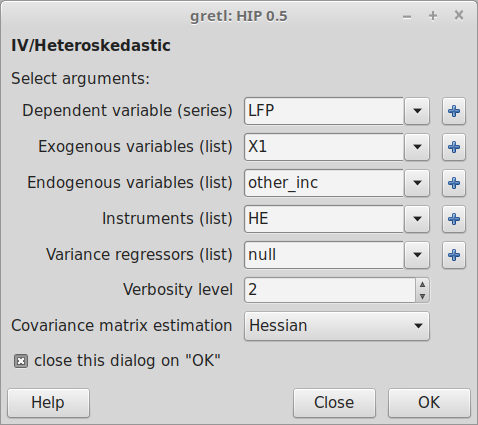
\includegraphics[scale=0.4]{HIP-sshot1.png}
  \caption{HIP GUI hook}
  \label{fig:HIP_window}
\end{figure}

After installing \HIP\, by going to \emph{Help $>$ Check for addons},
you'll find it among the other function packages installed on your box
(\emph{Tools $>$ Function packages $>$ On local
  machine}). Double-click and edit the window that appears like in
Figure \ref{fig:HIP_window}.

\begin{figure}[htbp]
  \centering
  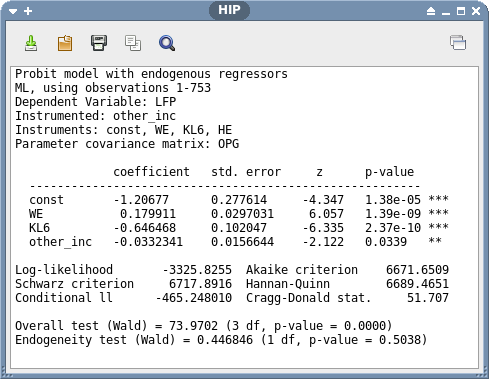
\includegraphics[scale=0.4]{HIP-sshot2.png}
  \caption{HIP output}
  \label{fig:HIP_output}
\end{figure}

\begin{figure}[hbtp]
  \centering
  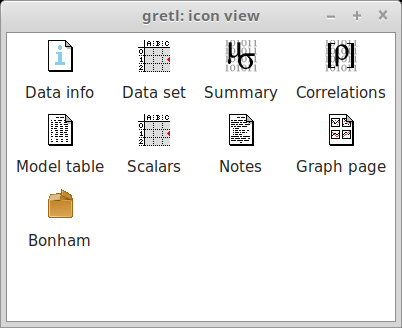
\includegraphics[scale=0.4]{HIP-sshot3.png}
  \caption{Icon view with a HIP bundle}
  \label{fig:iconview}
\end{figure}

Note that in this case we changed the default value of ``Verbosity''
from 1 to 2 and the default value of ``Covariance matrix estimation''
from ``OPG'' to ``Hessian''. 
%
% FIXME this does ot agree with Figures 1 and 2
%
This will have the effect of showing us the first stage
equation as well, and of using the Hessian instead of the OPG as the
method for computing standard errors. All this is apparent in Figure
\ref{fig:HIP_output}.

By using the \emph{Save} menu, you can choose the individual
elements of the bundle to store away for later use if you
want. Alternatively, you can save the bundle as a model via the
\emph{File $>$ Save to session as icon} menu entry. If you do, assuming
that you called your bundle ``Bonham'' again, then it will show in the
``Icon view'' gretl window, together with other session elements you
want to keep (see Figure \ref{fig:iconview}).

\subsection{Heteroskedastic probit}

Here, we'll replicate the example given in William Greene's textbook
(7th edition), which also uses \citeauthor{Mroz87}'s dataset. The
script goes like this:

\begin{code}
include HIP.gfn

open mroz87.gdt --quiet
series WA2 = WA^2
series KIDS = (KL6 + K618)>0
income = FAMINC /10000

list X = const WA WA2 income KIDS WE
list Z = income KIDS

Mitchell = HIP_setup(LFP, X, null, null, Z)
HIP_setoption(&Mitchell, "vcvmeth", 1)
 
set stopwatch
HIP_estimate(&Mitchell)
printf "Elapsed time = %g seconds\n", $stopwatch

HIP_printout(&Mitchell)
\end{code}

Note that in this case we did not use the \texttt{HIP} function, but
instead we split its workload between four separate functions:
\begin{description}
\item[HIP\_setup] Sets up the model: basically, it has the same
  parameters as the all-rounder \texttt{HIP} function seen
  above. Returns a bundle.
\item[HIP\_setoption] Set some details of the estimation procedure; in
  this case, we used it to compute standard errors using the inverse
  Hessian instead of the OPG matrix, so as to match exactly the
  figures reported in Greene's book.
\item[HIP\_estimate] Estimates the model: takes as argument the bundle
  address, plus an optional scalar for the verbosity.
\item[HIP\_printout] Prints out the results contained in the bundle.
\end{description}

This division of tasks may be convenient at times, because it gives
you finer control over ``what happens if''. For example, the
Cragg--Donald statistic gets computed during the initialization of the
bundle and you may wish to decide whether to proceed with estimation
or not depending on how strong your instruments are.

The output, replicating table 17.7 in Greene's textbook, should look
like this:

\begin{code}
Heteroskedastic probit model 
ML, using observations 1-753
Dependent Variable: LFP 
Parameter covariance matrix: Hessian

             coefficient   std. error     z      p-value
  ------------------------------------------------------
  const      -6.02985      2.49810      -2.414   0.0158  **
  WA          0.264291     0.118159      2.237   0.0253  **
  WA2        -0.00362838   0.00143387   -2.530   0.0114  **
  income      0.424441     0.221839      1.913   0.0557  *
  KIDS       -0.879093     0.302753     -2.904   0.0037  ***
  WE          0.140149     0.0518536     2.703   0.0069  ***

Variance 

             coefficient   std. error      z      p-value
  -------------------------------------------------------
  KIDS        -0.140752     0.323745    -0.4348   0.6637 
  income       0.312918     0.122810     2.548    0.0108  **

Log-likelihood        -487.6356  Akaike criterion     991.2712
Schwarz criterion     1028.2637  Hannan-Quinn        1005.5225

Overall test (Wald) = 14.5557 (5 df, p-value = 0.0124)
Heteroskedasticity test (LR) = 6.42453 (2 df, p-value = 0.0403)
Chesher and Irish normality test = 6.23055 (2 df, p-value = 0.0444)
\end{code}

\subsection{Let's get HIP. Heteroskedasticity and endogeneity at the
  same time.}

The script goes:
\begin{code}
set verbose off 
include HIP.gfn

open mroz87.gdt -q

list EXOG =  const WA CIT K618 
list ENDOG = WE
list ADDIN =  WMED WFED 
list HETVAR = HW 

Paice = HIP(LFP, EXOG, ENDOG, ADDIN, HETVAR, 2)
\end{code}

In this case, the ``2'' tells \HIP\ to be moderately verbose: don't
print out all the iterations, but show us the ``first stage''
coefficients. The output is as follows:

\begin{code}
Heteroskedastic probit model with endogenous regressors
ML, using observations 1-753
Dependent Variable: LFP 
Instrumented: WE
Instruments: const, WA, CIT, K618, WMED, WFED 
Parameter covariance matrix: OPG

             coefficient   std. error      z      p-value
  -------------------------------------------------------
  const      -0.551804     1.36344      -0.4047   0.6857 
  WA         -0.0304390    0.0172559    -1.764    0.0777  *
  CIT        -0.0242784    0.208991     -0.1162   0.9075 
  K618       -0.0927252    0.0896549    -1.034    0.3010 
  WE          0.199646     0.101330      1.970    0.0488  **

Variance 

             coefficient   std. error     z     p-value
  -----------------------------------------------------
  HW          0.117934     0.0571806    2.062   0.0392  **

"First-stage" regressions

             coefficient   std. error     z      p-value 
  -------------------------------------------------------
  const       9.68554      0.586171     16.52    2.49e-61 ***
  WA         -0.0159435    0.0104384    -1.527   0.1267  
  CIT         0.495907     0.152627      3.249   0.0012   ***
  K618       -0.136765     0.0612498    -2.233   0.0256   **
  WMED        0.180089     0.0265972     6.771   1.28e-11 ***
  WFED        0.168085     0.0253072     6.642   3.10e-11 ***

Log-likelihood       -2069.9119  Akaike criterion    4167.8239
Schwarz criterion     4232.5608  Hannan-Quinn        4192.7637
Conditional ll      -494.848818  Cragg-Donald stat.    103.337

Overall test (Wald) = 6.36207 (4 df, p-value = 0.1737)
Endogeneity test (Wald) = 0.509859 (1 df, p-value = 0.4752)
Test for overidentifying restrictions (LM) = 9.15786 (1 df, p-value = 0.0025)
Heteroskedasticity test (Wald) = 4.25379 (1 df, p-value = 0.0392)
\end{code}

\section{Computational details}

\HIP\ uses the analytical score and BFGS as the preferred optimization
method. The analytical Hessian is not implemented yet, but may be in
the future.

Like other estimators that depend on numerical methods, \HIP\ can
sometimes run into numerical problems, leading to non-convergence. 
If this happens, here are some points to consider.

\begin{itemize}
\item Checking exactly what happens during maximization can be very
  informative; try setting the verbosity parameter to 3.
\item Scaling of the data (especially $\Endog$) can be an issue; we do
  our best, but hey, give us a hand (for example, multiply or divide
  by 1000 depending of the original scale of the data).
\item Weak instruments: in some cases, there's little that can be
  done; see for example the artificially-generated dataset contained
  in the \texttt{MonteCarlo.inp} example script, contained in the
  examples directory. We do some heuristics, but we're not omnipotent.
\end{itemize}

%\clearpage
\bibliography{HIP}

\clearpage
\appendix

% \section{Installation}
% \label{sec:intall}

% Put the \texttt{HIP.gfn} file into a directory where \app{gretl}
% can find it. An excellent choice is the subdirectory where
% \app{gretl} keeps ordinary function files, which is the
% \texttt{function} subdirectory of \app{gretl}'s main directory. You
% may find out what this corresponds to on your system by inspecting the
% content of the built-in string \texttt{gretldir}. For example:
% \begin{code}
% gretl version 1.9.0cvs
% Copyright Ramu Ramanathan, Allin Cottrell and Riccardo "Jack" Lucchetti
% This is free software with ABSOLUTELY NO WARRANTY
% Current session: 2010-06-10 15:37

% "help" gives a list of commands
% Type "open filename" to open a data set
% ? gretldir
%  gretldir
% /usr/local/share/gretl
% ? 
% \end{code}
% so the subdirectory to use is
% \texttt{/usr/local/share/gretl/functions} in this example.

% This would install \HIP\ on a system-wide basis. On a multi-user
% system, you may want to put \texttt{HIP.gfn} in a user-specific place:
% on Linux (and, we assume, OSX), that would be
% \texttt{\$HOME/gretl/functions/}; on Windows, a likely candidate is
% \texttt{"My
%   Documents}$\backslash$\texttt{gretl}$\backslash$\texttt{functions"}.

\section{The boring stuff}

For computational purposes, we reparametrize the model using the
Cholesky decomposition $\RfVar^{-1} = CC'$. Moreover, by defining the
quantities below it is possible to reparametrize the joint density in
a computationally convenient way:
\begin{eqnarray*}
  \nu_i & = & \frac{1}{\sqrt{1- \ScCov' \ScCov}}
  \left( \frac{\Expla'\ProbitPar}{\CondSig}  + \ScRfDist' \ScCov \right) \\
  \ScCov & = & C'\Covars \\
  \ScRfDist & = & C' \left(\Endog - \RfPar \ExoInst\right) \\
  \vRfPar & = & \mathrm{vec}\left(\RfPar\right) \\
  \vechC & = & \mathrm{vech}(C)
\end{eqnarray*}

The estimable parameters are $\theta' = \left[\ProbitPar', \VarPar',
  \vRfPar', \ScCov', \vechC' \right]$

\subsection{The loglikelihood}
\label{sec:loglik}

As usual in such models, we divide the loglikelihood for each
observation into a marginal and a conditional component:
\begin{eqnarray*}
  \ell_i & = & \ell^m_i + \ell^c_i \\
  \ell^c_i & = & \ln P(\Depvar | \ExoInst, \CSReg, \RfDist) \\
  \ell^m_i & = & \ln f(\RfDist | \ExoInst, \CSReg) 
\end{eqnarray*}

The marginal component is nothing but an ordinary Gaussian
loglikelihood:
\[
\ell^m_i = -\frac{p}{2}\ln(2\pi) + \sum_{j=1}^p \ln c_{jj} - 
\frac{1}{2}\ScRfDist' \ScRfDist
\]
The conditional component is itself rather simple:
\begin{equation}
  \ell^c_i = \Depvar \ln\Phi(\nu_i) + \left(1-\Depvar\right)
  \ln \left[1-\Phi\left(\nu_i \right)\right]
\end{equation}
The only feature that sets $\ell^c_i$ apart from an ordinary probit
loglikelihood is that the index function depends non-linearly on some
of the parameters of the model, unless $\VarPar$ and $\ScCov$ are both
zero.

\subsection{The score}
\label{sec:score}

The analytical score will be derived in steps: first the marginal
component, then the conditional component. Of course, the chain rule
will be very useful.

Note first that the marginal component only depends on $\vRfPar$
(through $\ScRfDist$) and $\vechC$. Hence,
\[
\pder{\ell^m_i}{\vRfPar} = \pder{\ell^m_i}{\ScRfDist}
\pder{\ScRfDist}{\vRfPar} = \ScRfDist' \left( \ExoInst' \otimes C'
\right) =  \ExoInst' \otimes (C \ScRfDist)'
\]
and
\[
\pder{\ell^m_i}{\vechC} = \tilde{\mathbf{c}}' -
\ScRfDist'\pder{\ScRfDist}{\vechC} = \tilde{\mathbf{c}}' -
\left[\ScRfDist' \otimes (\Endog - \RfPar \ExoInst)' \right] S
\]
where $\tilde{\mathbf{c}}$ is defined as $\mathrm{vech}\left[ (I \odot
C)^{-1} \right]$ and $S$ is a selection matrix $S = \pder{\mathrm{vec}(C)}{\mathrm{vech}(C)}$.

For the purpose of computing the score for the conditional component,
note that $\ell^c_i$ depends on the parameters only through the index
function $\nu_i$, so $\pder{\ell^c_i}{\theta}$ can be evaluated as
\[
\pder{\ell^c_i}{\theta} = \pder{\ell^c_i}{\nu_i}\pder{\nu_i}{\theta} ;
\]
define $\mu(\nu_i)$ as
\[
\mu(\nu_i) = \pder{\ell^c_i}{\nu_i} = \Depvar
\frac{\phi(\nu_i)}{\Phi(\nu_i)} - (1-\Depvar)\frac{\phi(\nu_i)}{1
  -\Phi(\nu_i)}
\]
which is the customary (signed) inverse Mills ratio. Then,
\begin{eqnarray*}
  \pder{\nu_i}{\ProbitPar} & = & \frac{1}{\CondSig \sqrt{1- \ScCov'
      \ScCov}} \Expla' \\
  \pder{\nu_i}{\VarPar} & = & \pder{\nu_i}{\CondSig}
  \pder{\CondSig}{\VarPar} =
  \left[- \frac{\Expla'\ProbitPar}
    {\CondSig^2 \sqrt{1- \ScCov' \ScCov}} \right] \CondSig \CSReg' =
  - \left( \frac{\Expla'\ProbitPar}
    {\CondSig \sqrt{1- \ScCov' \ScCov}}\right)  \CSReg' \\
  \pder{\nu_i}{\ScCov} & = &
  \frac{1}{\CondSig^2 (1- \ScCov' \ScCov)}
  \left[ 
    \CondSig^2 \sqrt{1- \ScCov' \ScCov} \ScRfDist' - 
    \frac{\CondSig^2}{2} \nu_i (-2 \cdot \ScCov')
  \right] =
  \frac{ \ScRfDist'}{\sqrt{1- \ScCov' \ScCov}} +
  \frac{\nu_i \ScCov'}{1- \ScCov' \ScCov} \\
  \pder{\nu_i}{\vechC} & = & \frac{\ScCov'}{\sqrt{1- \ScCov'
      \ScCov}} \pder{\ScRfDist}{\vechC} \\
  \pder{\nu_i}{\vRfPar} & = &\frac{\ScCov'}{\sqrt{1- \ScCov'
      \ScCov}} \pder{\ScRfDist}{\vRfPar} = 
      - \frac{\ScCov'}{\sqrt{1- \ScCov' \ScCov}} \left( \ExoInst'
        \otimes C' \right) = 
      \frac{1}{\sqrt{1- \ScCov'\ScCov}} \left[ \ExoInst' \otimes (C\ScCov)' \right]
\end{eqnarray*}

As a consequence, the score with respect to $\vechC$ and $\vRfPar$ may
be written as
\begin{eqnarray*}
  \pder{\ell_i}{\vechC} = \pder{\ell^m_i}{\vechC} +
  \pder{\ell^c_i}{\vechC} &=&
  \tilde{\mathbf{c}}' +
  \left( \frac{\ScCov'}{\sqrt{1- \ScCov'\ScCov}} - \ScRfDist'\right)
  \pder{\ScRfDist}{\vechC} = \\
  & = & \tilde{\mathbf{c}}' +
  \left( \frac{\ScCov'}{\sqrt{1- \ScCov'\ScCov}} - \ScRfDist'\right)
  \left[I \otimes (\Endog - \RfPar \ExoInst)' \right] = \\
  & = & \tilde{\mathbf{c}}' +
  \left[
    \left( \frac{\ScCov'}{\sqrt{1- \ScCov'\ScCov}} - \ScRfDist'\right)
    \otimes (\Endog - \RfPar \ExoInst)' 
  \right] \\
\end{eqnarray*}

\section{List of functions}
\label{sec:syntax}
\subsection{Model setup}
\label{sec:gig_setup}

\begin{funcdoc}{HIP\_setoption(bundle *b, string opt, scalar value)}
  \begin{description}
  \item[Return type]: \texttt{scalar}
  \item[\texttt{b}]: pointer to a bundle containing the model to be
    estimated, as created by \cmd{HIP\_setup}; 
  \item[\texttt{opt}]: string, the option to set;
  \item[\texttt{value}]: scalar, the option value
  \end{description}

  This function sets up an option for estimation of the model, so it
  is typically used after \cmd{HIP\_setup} and before
  \cmd{HIP\_estimate}. At present, the possible values for the
  \texttt{opt} field are ``verbose'' (possible values: 0 to 3) and
  ``vcvmeth'' (possible values: 0 to 2).

  For ``verbose'', the meaning is: 0 = operate silently, 1 = standard
  output (default choice), 2 = print the first stage too for IV
  estimation and 3 = print out ML iterations.  For ``vcvmethod'', the
  meaning is: 0 = OPG (default), 1 = Hessian, 2 = Sandwich-robust.
\end{funcdoc}



\begin{funcdoc}{HIP\_setup(series y, list EXOG, list ENDOG[null], list ADDIN[null], \\
			  \rule{2cm}{0pt} list HETVAR[null])}
\begin{description}
  \item[Return type]: \texttt{bundle}
  \item[\texttt{y}]: a series containing $y_i$, the dependent binary
    variable; \textbf{(required)}
  \item[\texttt{EXOG}]: a list containing the exogenous variables
    $\Exog$ in $\ExoInst$ in equation \eqref{eq:main}; \textbf{(required)}
  \item[\texttt{ENDOG}]: a list containing the exogenous variables
    $\Endog$ in equations \eqref{eq:main}--\eqref{eq:RF}
  \item[\texttt{ADDIN}] a list containing the additional instruments $\Inst$ in $\ExoInst$
    in equation \eqref{eq:RF}
  \item[\texttt{HETVAR}] a list containing the variables $\CSReg$ of
    the skedastic function in equation \eqref{eq:main}
  \end{description}

  This function sets the model up so that it can be subsequently
  estimated via \cmd{HIP\_estimate}.
\end{funcdoc}

\subsection{Estimation}
\label{sec:syntax_estim}

\begin{funcdoc}{HIP\_estimate(bundle *b)}
\begin{description}
  \item[Return type]: \texttt{scalar}
  \item[\texttt{b}]: a model bundle in pointer form, as created by
    \cmd{HIP\_setup}.
  \end{description}

  General estimation function. It fills the bundle with the estimated
  coefficients and many other quantities of interest.
\end{funcdoc}

\subsection{Output}
\label{sec:syntax_output}

\begin{funcdoc}{HIP\_printout(bundle *b}
\begin{description}
  \item[Return type]: none.
  \item[\texttt{b}]: a model bundle in pointer form, as created by
    \cmd{HIP\_setup} and filled up by \cmd{HIP\_estimate}.
  \end{description}
  Prints out a model. Note: this function assumes that the bundle it
  refers to contains a model that has already been estimated. No
  checks are performed.
\end{funcdoc}

\subsection{GUI wrapper}
\label{sec:syntax_GUI}

\begin{funcdoc}{function bundle HIP(series y, list EXOG, list ENDOG[null],\ 
		    list ADDIN[null], list HETVAR[null], \
		    int v[0:3:1], int s[0:2:0])}
Using the same argument descriptions as \texttt{HIP\_setup}, after
checking the rank condition (if estimating instrumental variables
probit), it calls:
  \begin{enumerate}
  \item \texttt{HIP\_setup}
  \item \texttt{HIP\_setoption}
  \item \texttt{HIP\_estimate}
  \item \texttt{HIP\_printout}
\end{enumerate}
The parameter \cmd{v} controls the verbosity level: 0 = quiet, 1 =
main equation only, 2 = first stages, 3 = mle verbose.

\end{funcdoc}

\section{Bundle elements}
\label{sec:bundle_struct}
\begin{footnotesize}
\begin{tabular}{rlp{0.7\textwidth}}
  \hline
  \textbf{Name} & \textbf{Type} & \textbf{Purpose} \\
  \hline
  \multicolumn{3}{c}{Model descriptors} \\
  \hline
  \texttt{n}    & scalar  & number of observations \\
  \texttt{het}  & scalar  & acting as a Boolean switch,
  Heteroskedastic probit \\
  \texttt{iv}   & scalar  & acting as a Boolean switch, 
  Instrumental Variables probit \\
  \texttt{T}    & scalar  & number of observations used \\
  \texttt{t1}   & scalar  & first observation used \\
  \texttt{t2}   & scalar  & last observation used \\
  \hline
  \multicolumn{3}{c}{Data} \\
  \hline
  \texttt{depvar} & series  & dependent variable \\
  \texttt{mEXOG}  & matrix  & exogenous regressors \\
  \texttt{mk1}    & matrix  & number of exogenous regressors \\
  \texttt{mENDOG} & matrix  & endogenous regressors \\
  \texttt{mp}     & matrix  & number of endogenous regressors \\
  \texttt{mADDIN} & matrix  & additional instruments \\
  \texttt{mk2}    & matrix  & number of additional instruments \\
  \texttt{mHETVAR}& matrix  & variance regressors \\
  \texttt{mq}     & matrix  & number of variance regressors \\
  \texttt{mZ}     & matrix  & total regressors \\
  \texttt{mh}     & matrix  & number of total regressors \\
  \texttt{mX}     & matrix  & total instruments \\
  \texttt{mk}     & matrix  & number of total instruments \\
  \hline
  \multicolumn{3}{c}{Strings} \\
  \hline
  \texttt{depvarname}  & string & dependent variable name\\
  \texttt{mEXOGnames}  & string & exogenous regressors names \\
  \texttt{mENDOGnames} & string & endogenous regressors names \\
  \texttt{mADDINnames} & string & additional instruments names \\
  \texttt{mHETVARnames}& string & variance regressors names \\
  \texttt{mZnames}     & string & total regressors names \\
  \texttt{mXnames}     & string & total instruments names \\
  \hline
  \multicolumn{3}{c}{Estimation parameters} \\
  \hline
  \texttt{vcvtype}  & scalar & acting as an integer, method for estimating the 
  covariance matrix: 0 = OPG (default), 1 = empirical Hessian, 2 =
  Sandwich \\
  \hline
\end{tabular}
\end{footnotesize}


\begin{footnotesize}
\begin{tabular}{rlp{0.7\textwidth}}
\hline
  \multicolumn{3}{c}{Estimation results} \\
  \hline  
  \texttt{errcode}   & scalar & error code from \texttt{catch} \\
  \texttt{uhat}      & series & first stage residuals
  \citep{RiversVuong1988} \\
  \texttt{rescale}   & matrix & square root of the diagonal elements
  of first stage residuals covariance matrix \\
  \texttt{lnl0}      & scalar & second stage log-likelihood 
  \citep{RiversVuong1988} \\
  \texttt{theta}     & matrix & coefficients \\
  \texttt{VCVtheta}  & matrix & covariance matrix \\
  \texttt{lnl1}      & scalar & log-likelihood  \\
  \texttt{lnl1m}     & scalar & marginal log-likelihood  (if
  \texttt{iv})\\
  \texttt{lnl1c}     & scalar & conditional log-likelihood  (if
  \texttt{iv})\\
  \texttt{llt}       & series & log-likelihood  \\
  \texttt{SCORE}     & matrix & score matrix by observation  \\
  \texttt{infocrit}  & matrix & information criteria  \\
  \hline

  \multicolumn{3}{c}{Diagnostics\footnote{
      every diagnostic is saved in the bundle as a row vector of
      three elements: test statistic, degrees of freedom, p-value}} \\
  \hline  
  \texttt{WaldAll}   & matrix & Wald overall test \\
  \texttt{WaldEnd}   & matrix & Wald endogeneity test \\
  \texttt{LMOverid}  & matrix & LM test for overidentifying
  restrictions\\
  \texttt{HETtest}   & matrix & if \texttt{iv} Wald test, else LR test
  of Heterosckedasticity \\
  \texttt{CraggDondald} & scalar  & \cite{CraggDonald1993} statistic
  for weak instruments\\
  \texttt{normtest}  & matrix & Conditional moment test for normality
  of $\varepsilon_i$ \cite{ChesherIrish1987} \\
\hline
\end{tabular}
\end{footnotesize}

\end{document}


%%% Local Variables: 
%%% mode: latex
%%% TeX-master: t
%%% End: 

